% Template for PLoS
% Version 1.0 January 2009
%
% To compile to pdf, run:
% latex plos.template
% bibtex plos.template
% latex plos.template
% latex plos.template
% dvipdf plos.template

\documentclass[10pt]{article}
\usepackage{amsmath}
\usepackage{amssymb}
\usepackage{graphicx}
\usepackage{color} % for revision purposes only, may be not present in the final file
% cite package, to clean up citations in the main text. Do not remove.
\usepackage{cite}
\usepackage{color}
\usepackage{indentfirst} %% LM: in order to indent the first paragraph of each section
\usepackage{url} %% LM: in order to include nice urls
\usepackage{booktabs} %% LM: nice tables...
\usepackage{subfigure} % LM: panels
% Use doublespacing - comment out for single spacing
%\usepackage{setspace}
%\doublespacing

\topmargin 0.0cm
\oddsidemargin 0.5cm
\evensidemargin 0.5cm
\textwidth 16cm
\textheight 21cm

\usepackage[labelfont=bf,labelsep=period,justification=raggedright]{caption}

\bibliographystyle{plos2009}% 


\makeatletter
\renewcommand{\@biblabel}[1]{\quad#1.}
\makeatother


% Leave date blank
\date{}

\pagestyle{myheadings}
%% ** EDIT HERE **


%% ** EDIT HERE **
%% PLEASE INCLUDE ALL MACROS BELOW

%% END MACROS SECTION

\begin{document}

% Title must be 150 characters or less
\begin{flushleft}
{\Large
\textbf{Spatiotemporal Dynamics of Foot-and-mouth Disease Virus in South America}
}
% Insert Author names, affiliations and corresponding author email.
\\
Luiz Max Fagundes de Carvalho$^{1\ast}$,
Guy Baele$^{2}$,
Nuno Rodrigues Faria$^{2,3}$,
Andres M. Perez$^{4}$,
Philippe Lemey$^{2}$,
Waldemir de Castro Silveira$^{1}$
\\
\bf{1} Pan American Center for Foot-and-Mouth Disease (PAHO/WHO), Duque de Caxias, Rio de Janeiro, Brazil
\\
\bf{2} Department of Microbiology and Immunology, Rega Institute, KU Leuven, Belgium
\\
\bf{3} Department of Zoology, University of Oxford, Oxford OX1 3PS, UK
\\
\bf{4} Center for Animal Disease Modeling and Surveillance, University of California at Davis, Davis, United States of America
\\
$\ast$ E-mail: lcarvalho@paho.org
\end{flushleft}

% Please keep the abstract between 250 and 300 words
\section*{Abstract}

JUST IN THE END :)\\

Key-words: Phylogeography, foot-and-mouth disease virus, South America, animal trade, BEAST.

\section*{Introduction}

Foot-and-mouth disease virus (FMDV) is a rapidly evolving picornavirus, causative agent of the most important disease of domestic and wild cloven-hoofed animals, foot-and mouth disease (FMD) \cite{review}.
FMD is endemic in several regions of South America, and in recent years, the circulation of three of the seven FMDV serotypes, namely serotypes C, A and O, has been reported in the continent, the later two being the most prevalent.
%NRF perhaps you can drop here some references about serotype distribution in SAmerica
Serotypes A and O show different  geographic distribution, with O being more prevalent in endemic Andean areas \cite{andean} and A being responsible for sporadic emergences in the Southern cone \cite{Perez2001,Malirat2012}.
%NRF emergences=outbreaks?
FMDV has probably been introduced in South America in the early days of European colonization.
%NRF Reference missing here, perhaps include here Knowles and Samuel 2003, Tuly and Fares 2008. From my brief incursion into FMDV bibliography, it does look more that FMDV was introduced in the late days of European colonization (1860s, 1870s). If you want to re-address this question, perhaps you could include FMDV strains from European countries, but I think this question could potentially deviate the attention from main results presented here.
Large outbreaks, however, were not observed until the end of the 19th century.
%NRF I assume you're talking about outbreaks in South America, so do you mean 20th century?
By the 1970's, FMD was widespread in South America, with occurrence of multiple subtypes  in large-scale outbreaks \cite{Saraiva2003}.
As a consequence of the improving knowledge about disease ecosystems accumulated by the national programmes, the Hemispheric Plan for the Eradication of FMD (PHEFA) was launched in 1987. PHEFA was elaborated and signed by South American countries as a continent-wide programme to strenghten national infra-structures, control animal trade and improve diagnostic and epidemiological investigation capabilities \cite{review_eradication}. Its main objective is to create and maintain FMD-free areas, thus improving the availability of meat, milk and other economically important livestock products \cite{Saraiva2003,Saraiva2004,review_eradication,combining}. Considerable success has been achieved over the past years, with substantial reduction of FMD incidence in the late 1990's. Nevertheless, episodic outbreaks in 2001, 2005 and 2011 in previously free areas represented a serious setback to PHEFA, which was devised to fulfill its goals by 2010 \cite{Saraiva2003,Saraiva2004}.

The generally accepted solution to the problem of FMD eradication involves the promotion of transnational massive vaccination programmes \cite{vaccinationSA}
%NRF and strenghtening of co-operation between national governments and the private sector
%NRF I'd remove this from here or perhaps bring it to the discussion. It takes a bit the focus on the role of the veterenary surveillance systems and distracts from the role fo phylogenetics in the latter (i've now added transational that could also do the trick) 
with the development of better veterinary surveillance systems. Phylogenetic analyses have already proved useful in the latter, particularly by recovering in real-time the transmission pathways from genetic data \cite{cottam2008} and providing insight into the processes that drive re-emergence \cite{combining}.
In the South American ecotone, the molecular evolution of FMDV has been subject of several studies along the years \cite{Perez2001,Malirat2007,andean,Malirat2011,Maradei2013}.
These studies have played an important role in understanding the (re-)emergence pattern of FMDV, allowing for inference on the origin and evolutionary history of emerging viral strains \cite{topotypes,Perez2001}. Together with vaccine matching and MAb profiling studies \cite{Maradei2011}, phylogenetic analyses are a powerful 
tool to evaluate control programmes and guide vaccine formulation \cite{Maradei2011,Maradei2013}.

The increased availability of geo-referenced time-stamped genetic data has fostered the development of new methods that integrate epidemiological and environmental data in order to reconstruct pathogen population dynamics and test evolutionary hypotheses \cite{MEP,grenfell}. 
However, and as pointed out by Di Nardo, Knowles \&  Paton (2011) \cite{combining}, this joint evaluation of information from different sources is usually done outside of a unified quantitative framework, and in a qualitative fashion. In this context, Bayesian phylogeography offers a statistical framework to jointly combine multiple sources of information in order to understand the spatio-temporal dynamics of FMDV and perform evolutionary hypothesis testing. Such framework recently proven useful when investigating the patterns of FMDV spread and trace the spatial origins of FMD epidemics \cite{Carvalho2012,bulgaria,phymal}.

In this study we apply state-of-art Bayesian phylogeographic methods
%N implemented within the BEAST \cite{BEAST} package,
to investigate the evolutionary dynamics of serotypes A and O in South America, both in a spatial and temporal perspective. The probabilistic framework used here allows for the incorporation of multiple sources of information to test hypothesis about viral dispersal, while naturally accommodating uncertainty \cite{roots,towards}.
We use BEAST \cite{beast2012} 
%N citing here the most recent BEAST version instead
to build time-structured phylogenies and a recent demographic growth model \cite{skygrid} to reconstruct past population dynamics, to which we overlay with vaccination and serotype-specific notification data.
Moreover, we use data on livestock trade and geographical distances as predictors for viral spatial diffusion and use recently developed methods to accurately calculate marginal likelihoods for each predictor.
Finally, we offer an appreciation of the statistical hurdles that may be caused by biased geographic sampling, and propose ways to ameliorate their effects.

% Results and Discussion can be combined.
\section*{Results}

\subsection*{South American FMDV serotypes A and O exhibit rate variation among lineages and evolve measurably}

In this study, we analyzed all publicly available VP1 (1D) sequences for serotypes A and O in South America (131 and 167 sequences, respectively) using a Bayesian phylogeographic approach. Our data sets spanned over a large period (1955-2010 for serotype A and 1994-2010 for serotype O)  and covered nearly all South American countries affected by FMD.

%NRF This sentence should probably go to discussion: 
%Bayesian phylogenetics provides a framework for rigorously testing evolutionary hypotheses without conditioning on a single tree topology. Hence, this approach naturally accommodates phylogenetic uncertainty and, combined with accurate methods for marginal likelihood calculation, perform Bayesian model selection \cite{Baele2012,Baele2013a,Baele2013b}.

%NRF This sentence should probably go to discussion too: 
%This continent wide-sampling allowed us to reconstruct the temporal and spatial dynamics of FMDV in the continent for both serotypes in greater detail than previous studies.

%NRF This sentence should probably go to Materials and Methods:  

First, jModelTest selection analysis yielded the general time reversible (GTR) model with a discretized gamma distributed across-site rate variation and a proportion of invariant sites (GTR+I+$\Gamma_{4}$) model as the best fit nucleotide substitution model for both FMDV data sets. Next, we performed a stringent model selection analysis to chose the best-fit demographic growth model and molecular clock model. Our results indicate that the constant population assumption is decisevely rejected (A: BF=$11$; O: BF= $21$) in favour of a model that allows fluctuations in demographic growth over time. 

After, we estimated that both sertoypes A and O rapid evolution better fits a relaxed than strict molecular clock model. Particularly, the exponential relaxed molecular clock provided a better fit for serotype O data (BF=$21$) while the lognormal relaxed molecular clock model provided a better fit to serotype A (BF=$11$) (see Table S1 for details). The coefficient of variation for the relaxed molecular clock models was estimated at xx (95\% BCI: xx) and xx (95\% BCI: xx) respectively for serotype A and O, indicating substantial rate heterogeneity among lineages in the phylogeny. 

We also performed a 'temporal signal' test to evaluate the degree to which genetic divergence accumulates over time (described in \cite{Faria2012}). This confirmed significant temporal signal for both serotypes (A: BF=$310$; O: BF=$348$), showing that both FMDV data sets analysed here are measurably evolving populations. Overall, these results show that sufficient temporal information is embedded in sequence data of both serotypes under investigation, which is central for the estimation of times of divergence and to reconstruct the population dynamics in natural time units \cite{MEP}.

\subsection*{Dating the divergence of FMDV in South America}

%NRF Changed mutation to evolutionary rate since mutation rate (rate at which errors are incorporated in the genome, estimated in wet lab) is different from evolutionary or substitution rate (rate at which mutations spread and become fixed in a population, estimated from seq data). Do the 'mutation rates' that you cited in the 'review' paper for serotype O correspond to evolutionary rates? (mutation rate is generally > evolutionary rate).

To build time-structured phylogenies for each FMDV serotype, we performed Bayesian MCMC analysis using BEAST, under the corresponding best-fit combination of nucleotide subsitution, demographic and molecular clock models.

The maximum clade credibility (MCC) tree estimated for serotype A (Figure~\ref{fig:Atree}) 
%shows a time to most common recent ancestor (TMRCA) of around 75 years, 
places the origin of the circulating strains in or around the early years of the 1920's decade.
This result is surprising, since it reveals a longer-term maintenance of FMDV serotype A in the continent than previously suspected.
%NRF Not so sure if this is very updated... check Tuly and Fares, Virology, 2008
Figure~\ref{fig:Atree} shows that sequences from the same country tend to cluster in small clades although the Bayesian phylogenies for both serotypes also shows considerable interspersing of lineages indicating trans-border FMDV migration. For example, for serotype A sequences from Argentina are grouped in 2 clades that either comprised only Argentinian isolates or include sequences from Brazil and Uruguay (Figure 1). Interestingly, the great majority of the isolates from Venezuela and Colombia fall together within 2 distinct clades. 

\begin{center}
 [Figure 1 about here]
\end{center}

Figure~\ref{fig:Otree} presents the estimated MCC tree for serotype O. The same interspersing trend can be noticed, with Ecuador and Colombia showing several interleaved clades. The TMRCA for serotype O was estimated in around 20 years, showing a more recent origin. Here, a smaller clade of Colombian isolates are found interspersed within from Venezuelan isolates. In addition, isolates from Ecuador are found interspersed with isolates from Colombia, suggesting that the intra-country dynamics of FMDV between these two countries is intrinsically linked. Overall, the Bayesian phylogenies suggest that most FMDV flow within South America occured between neighboring countries. 

Using the best fitting demographic and molecular clock model combination for each serotype, the evolutionary rate for serotype A was estimated around $4 \times 10^{-3}$ substitutions/site/year. In addition, the estimated evoltutionary rate for serotype O was aproximately 2.5 times faster than serotype A, i.e. at $1 \times 10^{-2}$, consistent with previous studies \cite{review,Carvalho2012}. 

\begin{center}
 [Figure 2 about here]
\end{center}

%NRF Just a suggestion: we could also show Figure 1 and 2 as Figure 1 panels A and B, side by side, with a single shared legend
%NRF I am also wondering if we should also add some posterior values to the trees (and to the text)

\subsection*{Spatial Dynamics of FMDV in South America}

% in the table (I'd merge Tables 1 and 2 into 1 single Table), include a note mentioning that you are only showing the MC statistics for the countries for which there were at least 3(5?) sequences. It is a bit odd that for serotype A, Peru and Ecuador do not have a significant p-value, but that serotype O has significant structure in Ecuador - this is clearly reflecting the fact that for O there is only 1 sequence for Ecuador. Should we have more data from Ecuardor and we 'd probably find structure of O there as well.

To assess the spatial pattern of FMDV spread within South America, we performed Bayesian phylogeographic analysis, also using the models available in BEAST \cite{roots}.
We began by evaluating the spatial signal contained in our sequences using Bayesian tip-association tests \cite{bats} to determine the amount of spatial signal in our reconstructed phylogenies.
To gain insight into the amount of association for each location, we computed the maximum clade (MC) statistic.
The results for serotype A are presented in Table~\ref{tab:BaTSA} and results for serotype O can be found in Table~\ref{tab:BaTSO}.
For both serotypes, we observed significant location-tip association.
MC statistics were different for each country in each dataset, showing different geographic structures for each serotype.
As an overall result, our datasets presented high degree of spatial signal, what justifies more complex phylogeographic analyses to study the transmission network of FMDV in the continent.

Fist, we employ an asymmetric continuous-time Markov chain (CTMC) phylogeographic model \cite{roots} to gain insight into the spatio-temporal process of FMDV spread.
The results are presented in Figure ~\ref{fig:migration} and show that Brazil and Colombia were the most probable origins for serotypes A and O respectively.

We can notice that for serotype A mainly long-range migration routes were inferred for the period before 1945.
This results may be due to sparsity of information before 1970, which precludes accurate inference about periods further back in time. 
Also, there is a major expansion in spatial spread from 1945 to 1965, characterized by Brazil as a source of virus for the rest of the continent.
In the period 1965-1980, we notice slower spread, mainly through short range routes.
The 1980-2008 window is characterized by the introduction of FMDV serotype A in Peru and Paraguay and the increase of intra-country diversity (depicted by the radius of the displayed circles).   

On the other hand, for serotype O expansion seems to have occured by the middle of the 1990 decade.
Up to 1995, Colombia and Brazil seem to have acted as primary and secondary viral sources, respectively.
From 1995 to 2000, whilst Colombia acted as main source for the northern/andean regions of the continent, spread in the Southern Cone seems to originate in Brazil.
The period 2000-2010 is characterized by a decrease in viral flow (almost no new edges added to the network) and the main feature is the increase in viral diversity within countries, specially Ecuador, Colombia and Brazil.
	
To further explore the spatial behavior of FMDV we employ the so-called ``Markov jump'' counts \cite{Minin2008} of the expected number of location state transitions along the  branches of the phylogeny, which  provide a quantitative measure of gene flow between countries, representing successful viral introductions from one region to another.

Coupled to this analysis we set up a Bayesian Stochastic Search Variable Selection (BSVSS) procedure to search for the most parsimonious set of migration routes (network edges) needed to explain the diffusion process (see Methods).
BSSVS also naturally allows for the computation of Bayes factors, which are in turn used to assess the importance/significance of each migration path.
The results of this analysis are presented in Figures ~\ref{fig:mj&BFs} and show that supported migration routes differ for each serotype, with some overlapping in the routes connecting Venezuela, Colombia and Ecuador.

Notably, Venezuela, Colombia and Ecuador form a densely connected sub-network for both serotypes.
% Lots of short range routes are supported for both serotypes 
To further study this pattern, we compared the counts between countries that share borders and those which do not. The results show ... % TODO: actually do this analysis

One may ask if both serotypes present different spatial spread patterns.
To assess this we used PS/SS to calculate marginal likelhihoods for two different models, henceforth  called "shared'' and "separate''.
In the "shared'' model we used trait (location) and sequence data  from both serotypes to make inference about one CTMC rate matrix, whilst in the "separate'' model we allow both serotypes to have each one CTMC rate matrix, while using the combined data from both serotypes.
Both models allow serotypes to have different spatial diffusion rates.


\begin{center}
 [THIS SECTION IS UNDER MAJOR REVIEW]
\end{center}

\subsection*{Identifying potential predictors of FMDV spread in South America}
The ability to incorporate multiple sources of information like temporal and spatial data is becoming increasingly important in molecular epidemiology studies that aim to understand the driving forces of pathogen evolution and spread \cite{towards,combining,MEP,roots}. 

We used data from the detailed trade matrix available from the Food and Agriculture Organization (FAO) to elicit CMTC rate matrix priors (predictors), henceforth called here "trade-informed priors''.
By accurately calculating the marginal likelihood of each trade-informed prior we can gain insight into the importance of each predictor on viral spread \cite{Carvalho2012,Nelson2011}.
The results of this analyses, presented in tables ~\ref{tab:predA} and ~\ref{tab:predO}, showed that ... % I'm sure Guy has something to add here ;)

%NRF Do have any results for the analyses combining the rate matrices of O and A? What was the best fitting predictor  in this case?

\subsection*{Sampling bias assessment in the phylogeographic analysis}
% BSSVS across samples
% KL divergence across samples
% phylogenetic parameter estimates

\subsection*{Demographic reconstruction of FMDV dynamics}

The results from the Skygrid reconstruction show strikingly different dynamical behaviors for the two serotypes, with serotype O exhibiting considerable more oscillation over time, and a diversity peak occurring in late years of the 1990 decade.
Serotype A exhibits a more stable behavior over most of the 20th century, with most variation occurring within the temporal sampling interval, mainly in the last years of the 2000 decade.
To better understand the relationship between vaccination and viral diversity, we overlaid vaccination data to our skygrid plots presented in Figure~\ref{fig:skygrid}.
These data were expressed as doses per head, which we consider to be a more accurate measure of vaccination coverage, since it corrects for population size increase/decrease over time (see SFigure 1 for livestock population and trade time series).
Also, serotype-specific disease notification data was collected and plotted as an overlaid time series to the reconstruction. 

\begin{center}
 [Figure 3 about here]
\end{center}


\section*{Discussion}
%  Interestingly, best fit branch substitution models (molecular clock) were different for both serotypes (Table S1) suggesting different evolutionary dynamics
Thus, while for serotype A a more restrictive exponential molecular clock and a slower mutation rate were found, for serotype O our results point out a more diffuse distribution of branch-specific substitutions (lognormal) and a faster evolutionary rate.
The differences in evolutionary rates, when taken together with the results from molecular clock model selection, suggest that, although the two serotypes share the same host and infection routes, they present rather different evolutionary dynamics. 

It can be noticed from both serotypes that over time, with the increase of vaccination coverage, viral effective population size ($Ne$) decreases dramatically.
This drop is also present in FMD notifications, what may suggest the role of epidemics in viral diversity.
These results draw an interesting picture: over the years vaccination seems to be disrupting viral diversity, supposedly by precluding spread over large spatial extents, inducing a state of focalized transmission [NEED A REF HERE].

In order to strenghten epidemiological inference, it may be interesting to compare the results obtained for both serotypes. Serotype O presents more estable temporal behavior, whereas serotype A is more fluctuating.
Previous studies have shown that occurences caused by serotype A present longer cycles and wider epidemics, while serotype O is more prevalent with shorter disease cycles \cite{colombiatime}.
These epidemiological features are reflected at the temporal variation observed for viral $Ne$ in both serotypes, a result obtained for other viruses as well \cite{Bennett2010,Pybus2003}. 
Since our results reinforce the notion that these two serotypes present different evolutionary dynamics, the overall decrease in viral diversity for both serotypes points towards a progressive success of the eradication programme in slowly reducing transmission and controlling epidemics.

Using animal trade data as predictors can be a valuable tool to understand the role of livestock commerce in the spread of animal and zoonotic diseases \cite{Nelson2011}.
We found significant well supported migration paths between Venezuela, Colombia and Ecuador for both serotypes and this may indicate...???% TODO: 
% These countries share borders and have similar enviromental conditions % TODO: do they?
% serotype A expansion took place mostly in the early years of the 20th century and expansion for serotype O occured in the beggining of the 1990 decade.
% We focus on a comparative approach, using information obtained from both serotypes to gain insight into the general process of FMDV spread in South America.
% Although both serotypes have different tempo, several spread routes were found in both migration networks. As an important difference...
% These results help to shed light into the main determinants of viral flow in the continent.
% While serotype A seems to have spread in a period of less stringent control, results for serotype O indicate that... % TODO Andres could help A LOT here! 
% the relationship between MJ borders inference and source-sink dynamics
% For serotype O, Colombia is north, Brazil is south.
% REMEMBER TO DISCUSS SHARED VERSUS SEPARATED ANALYSES. shared vs separated reveal that spatial spread is quite the same
% Informing the rates with livestock trade contributes to ameliorate the bias introduced by unbalanced sampling in the sense that it allows for an external source of information to be incorporated \cite{Faria2012}.
% Moreover, our results suggest that \ldots
% As discussed by Cottam et al (2007) \cite{cottam2007}, phylogenetic methods can be used to unravel undetected transmission.
%\textcolor{red}{Skygrid is specially suited to detect slight but meaningful variation in population effective sizes, allowing for more precise epidemiological inference}.\\



\section*{Conclusions}
%better methods yield more complete analyses
%overall decrease in viral diversity
%spatial routes by proximity
%sampling bias may be an important factor to consider 
\section*{Methods}

\subsection*{Genetic and epidemiological data}

To study the spatio-temporal spread dynamics of FMDV within South America we compiled the largest database of 1D (VP1) gene sequences to date for serotypes A and O.
We retrieved all 1D (VP1) nucleotide sequences available from the National Center for Biotechnology Information (NCBI, \url{ http://www.ncbi.nlm.nih.gov/}) for which there was information on country and year of isolation.
This resulted in 131 sequences (eight countries) for serotype A and 167 sequences (nine countries) for serotype O, covering time spans of 55 (1955-2008) and 16 (1994-2010) years, respectively (see Text S1 for details).
Each dataset was aligned using the MUSCLE algorithm implemented in the MEGA5 \cite{MEGA} package.
%NF cite also MUSCLE here 

Data on animal trade were obtained from the FAO database (\url{http://faostat.fao.org/}).
We retrieved data on the detailed trade matrix for cattle, pigs and sheep (live animals) covering the period from 1986 to 2009, for each of the nine countries.
Serotype-specific outbreak notifications were obtained from FMD Bioportal (\url{http://fmdbioportal.ucdavis.edu:8080/}).

\subsection*{Phylogenetic Analysis}

First, we checked both data sets for recombination using the tools (SBP and GARD \cite{sbpgard}) available from the Datamonkey facility (\url{http://www.datamonkey.org/}), and no recombination was found.
We then used hierarchical likelihood model selection, as implemented in the package jModeltest 0.1.1 \cite{jmodel}, to select the best nucleotide substitution model for each data set.
%NF I think this should be Results (moved it into there now)
%This analysis yielded the general time reversible (GTR) model with a discretized gamma distributed across-site rate variation and a proportion of invariant sites (GTR+I+$\Gamma_{4}$) model as the best fit for both data sets.

We performed Bayesian model selection to assess the performance of different demographic and molecular clock models.
To this end, we used state-of-the-art marginal likelihood estimators, such as path sampling (PS) \cite{LartillotPhilippe} and stepping-stone sampling (SS) \cite{Xie}, which have only recently been introduced in the field of phylogenetics.
Both PS and SS have been previously shown to outperform traditional posterior-based marginal likelihood estimators, such as the harmonic mean estimator (HME) and its stabilized version (sHME) \cite{LartillotPhilippe,Xie,Baele2012,Baele2013a,Baele2013b}.
Further, it has been shown that the use of proper priors is essential when performing Bayesian model selection \cite{Baele2013a}, and by extension, when conducting Bayesian inference through Markov chain Monte Carlo (MCMC).
                                                                       
%GB: Did we estimate marginal likelihoods for the skyride or for the skygrid? <- LM: skyride...
%NF: Would it be time consuming if we tested for the skygrid? 
%GB: Why did we not compare the UCED and UCLD to the STRICT clock? Should we still do that? <-LM: we did, indeed. updated

Using PS and SS, we have estimated the (log) marginal likelihood for several combinations of tree priors and molecular clocks, and this for each data set.
We compared the Skyride model, i.e. a Bayesian nonparametric model that parameterizes the effective population size as a piecewise constant function and employs a GMRF prior to smooth the trajectory \cite{skygrid}, to a constant population size model.
Further, we combined each of these demographic models with a relaxed molecular clock model, assuming either a lognormal or an exponential distribution to parameterize the rate distribution.
The results of these model comparisons can be found in Table S1.

Next, we employ Bayesian coalescent-based methods to build time-structured phylogenies for the two serotypes to gain insight into the past population dynamics of the virus.
We use this approach to determine the time to most recent common ancestor (TMRCA) for each data set using the BEAST \cite{BEAST} software package.
 Given the computational demands of these approaches, we use BEAST \cite{BEAST} in combination with BEAGLE \cite{BEAGLE} to increase computational efficiency.


\subsection*{Quantifying temporal and spatial signal} 

To assess the "temporal signal'' for each serotype, we took the approach of Faria et al (2012) \cite{Faria2012} and compared the marginal likelihoods of a "dated tips'' model and a contemporaneous tips model by calculating Bayes factors (BF) \cite{Suchard2001,KassRaftery1995} (see Spatial Model Selection for details).
We followed Kass and Raftery (1995) \cite{KassRaftery1995} and considered BF$>3$ to be indicator of decisive support for the hypothesis of temporal structure.

Spatial signal was quantified using Bayesian tip-association tests, implemented through the BaTS software package\cite{bats}.
Each sequence was assigned to its country of origin and we computed association index (AI) and parsimony score (PI).
Using a subset of 1000 samples from the posterior distribution of topologies, we obtained a null distribution for each statistic, against which the observed indexes were compared and significance was assessed.
Additionally, we computed the so-called monophyletic clade (MC) size for each state (country), as a local indicator of phylogeny-trait association for each state.


\subsection*{Temporal Dynamics}

We apply the recently developed Skygrid coalescent model \cite{skygrid} in order to reconstruct the past population dynamics for both serotypes. Skygrid is a nonparametric coalescent-based method that uses a Gaussian Markov Random Field (GMRF) prior to obtain smooth estimates for effective population size trajectories over time \ldots 

and then overlay the results to serotype-specific outbreak notifications.


\begin{center}
 [NUNO'S SHARE]
\end{center}


\subsection*{Spatial Analysis}

BEAST \cite{BEAST} implements a set of diffusion models for spatial spread, both for discrete and continuous data.
In this paper, we focus on the discrete case and model the diffusion process as a continuous-time Markov chain (CTMC) \cite{roots}, treating the country of sampling of each sequence as a discrete state.
To gain insight into the transmission network of FMDV in South America we apply an asymmetric non-reversible discrete phylogeography model to both data sets, with each country used as a discrete state.
For statistical efficiency, we employ Bayesian stochastic search variable selection (BSSVS) in order to choose the minimal set of rates that sufficiently explain the observed data.
BSSVS naturally allows for assessing the significance of each migration route, by calculating Bayes factors.
We used the SPREAD \cite{spread} package to annotate the results of all the spatial analyses presented in this paper, generating KML files (visualized using Google Earth, \url{http://www.google.com/earth/index.
html}) and calculate the BFs from BSSVS.

Taking advantage of the probabilistic nature of this framework, we also estimated net rates of migration and also tested the statistical fit of several predictors for viral spread (see Spatial Model Selection).

To estimate the rate of viral flow between countries, we used the Markov Jumps \cite{Minin2008} approach.
Estimation is done by keeping track of (counting) labeled transitions along each branch of the phylogeny.
This way, we can compute the expected number of transitions between each pair of locations conditional on the observed data.
These expectations can then be multplied by geographical distances to obtain the expected distance travelled within the time elapsed on each branch \cite{zoonotic}.


\subsubsection*{Spatial Model Selection}

One of the main research questions in this study is whether or not the two serotypes share the same underlying dispersal determinant. 
To test this hypothesis, we estimated one single CMTC rate matrix using data from both serotypes, while allowing each serotype to have its own dispersal rate. 
This option is justifiable, since the two serotypes present different TMRCAs and mutation rates. 
%The marginal likelihood of this model was compared to that of one in which both serotypes were allowed to share data from both alignments but estimate two separate rate matrices.

Another important aspect is the influence of different variables, such as population size and density, presence of airlines and roads and disease incidence on viral diffusion through space. 
The framework adopted here allows for the incorporation of such information into the inference process, by the suitable formulation of prior distributions to inform the entries of the rate matrix. 
To assess this, prior distributions were formulated using the following variables: trade of live cattle, pigs and sheep, as well as great-circle distances between each pair of countries. 
These variables were normalized such that their expectation was one with unit variance. See Figure S1 for kernel density smoothing of these prior distributions.

In this study, we exploit recent developments in Bayesian model selection \cite{Baele2012}, as implemented in the BEAST software program \cite{BEAST}.
Phylogenetics has adopted two main methods of potentially general applicability, such as importance sampling estimators (such as the HME and sHME) and path sampling estimators (such as PS and SS) to compute marginal likelihoods of competing models.
These approaches allow for an overall ranking of competing models to be constructed, from which the top-performing model can easily be determined.
Due to their ease of use and computational tractability, with collected likelihood samples from the standard MCMC run being re-used, the posterior-based (log) marginal likelihood estimators have received widespread adoption in the field of phylogenetics.
Whereas PS methods represent very general estimators and can also be applied to any model for which MCMC samples can be obtained, they are computationally demanding and require additional analyses to collect the necessary likelihood samples needed to estimate the (log) marginal likelihood.

Accurate estimation of (log) marginal likelihoods are crucial to correctly identify models that best describe the observed data. 
Using these (log) marginal likelihoods, it is possible to calculate Bayes Factors, which give a measure of the relative performance of each model. 
The stepping stone (SS) and path sampling (PS) approaches, as implemented in BEAST, were used  to calculate all marginal likelihoods reported in this paper.
Note that these approaches accommodate phylogenetic uncertainty.
PS and SS calculations were run using 64 power posteriors, each running for 500.000 iterations, taking up to 3 weeks of computation for each model under evaluation.




\subsection*{Assessing the effect of sampling}

As already found in previous studies \cite{Faria2012, Lemey2013}, unbalanced sampling can have an important impact on the inference of the spatial migration rates, as the rates from and to more represented locations tend to be overestimated[I NEED A REF FOR THAT].
In this study, both data sets analyzed presented highly preferential sampling, with Ecuadorian sequences representing about 50 \% of the serotype O data and about 45 \% of serotype A sequences being from Argentina.

To assess the impact of sampling in our estimates, we performed the following experiments:
\begin{itemize}
 \item i. Parameter estimation without the over-represented locations;
 \item ii. Parameter estimation with over-represented locations downsampled to the number of sequences of the second most represented location (Venezuela and Colombia, for serotypes A and O, respectively). For each serotype, we obtained five random subsamples using this approach;
 \item iii. Estimation of the marginal likelihood of a ``representation-informed'' prior distribution for the rates, detailed below.
\end{itemize}

In order to assess the relevance (impact) of the sampling scheme on the inference of the rate matrix, we formulated a representation-informed prior distribution, as follows: let $n_i$ and $n_j$ be the numbers of sequences available for locations $i$ and $j$, respectively.
 The representation-informed prior is a multivariate gamma prior, with expectations given by
\begin{equation}
 m_{ij}=C\frac{|n_i-n_j|}{\sum_i|n_i-n_j|}
\end{equation}
where $C$ is an arbitrary constant, chosen such that $E[m_{ij}]=1$.
To analyze experiment iii, we used BSSVS to estimate Bayes Factors and compared BFs obtained with different sub-samples.
Additionally, we computed Kullback-Leibler divergence \cite{KL,roots} of the root state distributions using a discrete uniform distribution as reference. 
% Do NOT remove this, even if you are not including acknowledgments

\section*{Acknowledgments}
The authors would like to thank Ant\^onio Mendes (PANAFTOSA) for clarifications regarding the vaccination data, Professor Marc Suchard (UCLA) for insightful contributions and Miguel Carvalho for operational support.
We acknowledge the support of the National Evolutionary Synthesis Center (NESCent) through a working group (Software for Bayesian Evolutionary Analysis).

\emph{Funding:} The research leading to these results has received funding from the European Union Seventh Framework Programme [FP7/2007-2013] under Grant Agreement no. 278433-PREDEMICS and ERC Grant agreement no. 260864.

\emph{Conflict of Interest:} none declared.

%\section*{References}
% The bibtex filename
\newpage
\bibliography{FMDV_AMERICA}
\newpage
\section*{Figure Legends}

{\bf Figure~\ref{fig:Atree}. Phylogenetic Relationships of 131 serotype A FMDV isolates from South America.} Time-scaled phylogenetic maximum clade credibility (MCC) tree for FMDV VP1 sequences from eight countries in the period 1955-2010 is presented. Tips were collapsed for clarity and colored according to geographic origin. Diamonds sizes are proportional to posterior probabilities.

{\bf Figure~\ref{fig:Otree}. Phylogenetic Relationships of 167 serotype O FMDV isolates from South America.} Time-scaled phylogenetic maximum clade credibility tree for FMDV VP1 sequences from eight countries in the period 1955-2010. Tips were collapsed for clarity and colored according to geographic origin. Diamonds sizes are proportional to posterior probabilities.

{\bf Figure~\ref{fig:skygrid}. Temporal dynamics of FMDV serotypes A and O in South America.} Population dynamics were reconstructed for both serotypes using the Skygrid model (see Methods). Additionally, data on vaccination  (doses per head) and (log) FMD serotype-specific notifications were superimposed on the demographic reconstruction, with 95 \% Bayesian Credible Intervals shaded in grey.

{\bf Figure~\ref{fig:mj&BFs}. Migration networks for FMDV serotypes A and O in South America.} We estimated the number of migration events between countries using Markov jumps.  Bayesian Stochastic Variable Search Selection (BSVSS) was used to determine most significant migration routes and Bayes factors are depicted by arrows, with line thickness proportional to BF magnitude. Coroplethic maps show the net migration rates for each country, for both serotypes.

{\bf Figure~\ref{fig:migration}. Spatiotemporal dynamics of FMDV in South America} Using an asymmetric diffusion model, we reconstructed the spatial spread of FMDV serotypes A and O throughout the South American continent during the XX century. Circle radius's are proportional to lineage diversity. Illustrations produced using data annotated from SPREAD \cite{spread} and vizualized using Google Earth (\url{http://www.google.com/earth/index.
html}).

{\bf SFigure~\ref{sfig:tradeinfo}. Kernel density estimation for the trade-informed priors used in this study}. Information on cattle, sheep and pigs trade was retrieved from FAO and used to create trade-informed prior distributions for the CTMC infinitesimal rate matrix. Each prior was evaluated for prior predictive probability (marginal likelihood) using the PS and SS algorithms.

\newpage
\section{Figures}
%%%%%%%%%%%%%%%%%%%%%%%%%%
%%%%%%%%%%%%%%%%%%%%%%%%%%
\begin{figure}[!ht]
\begin{center}
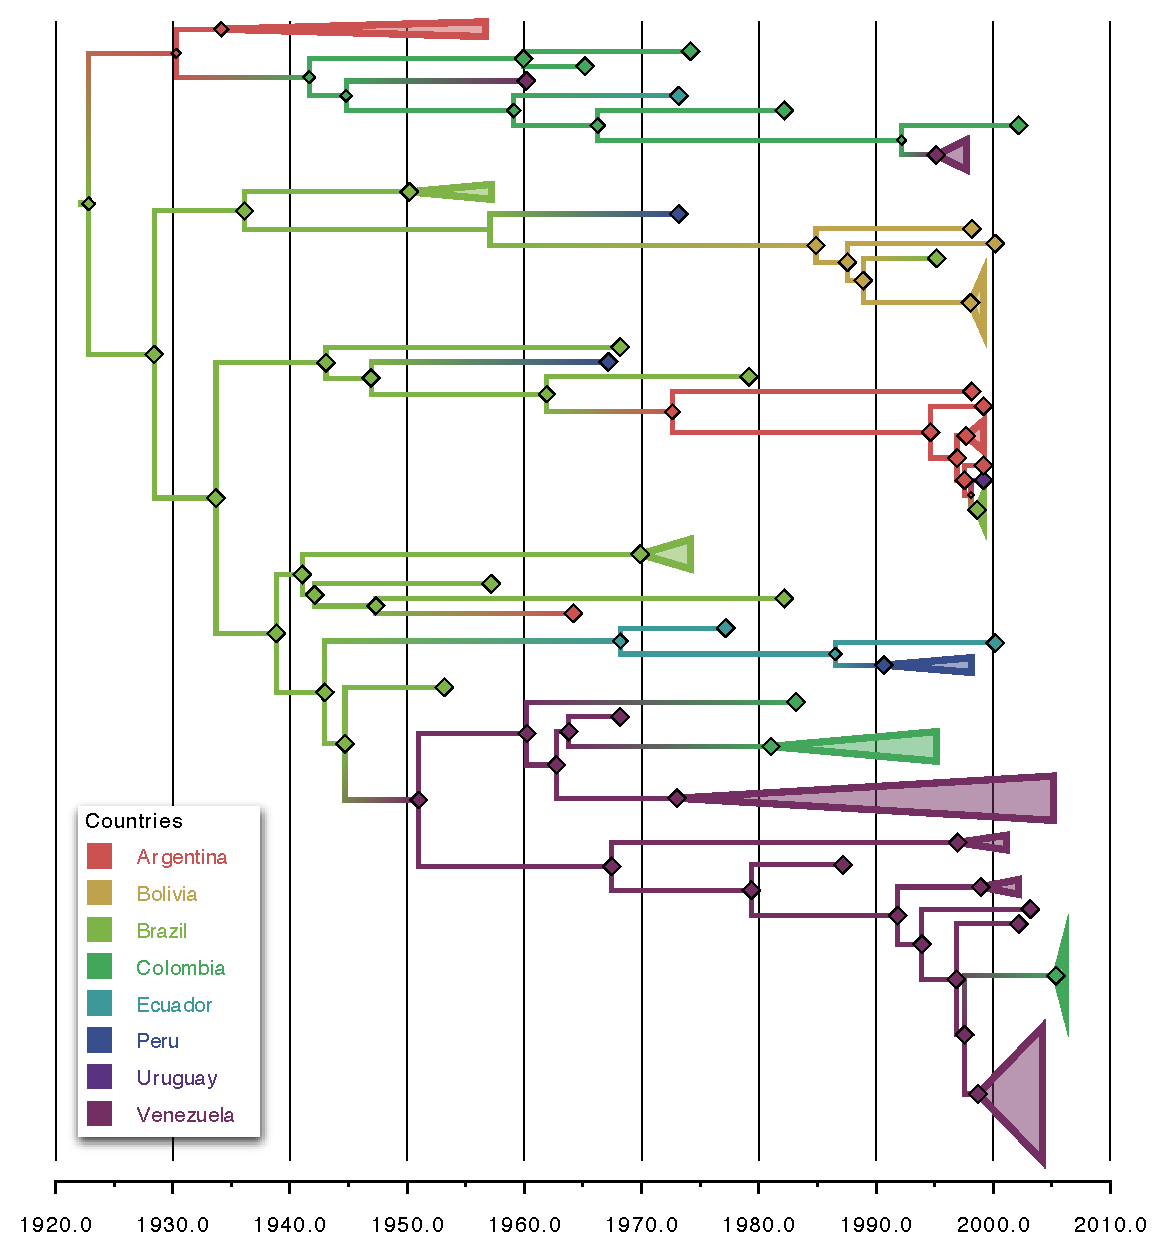
\includegraphics[scale=.85]{FIGURES/A.pdf}
\end{center}
\caption{}
\label{fig:Atree}
\end{figure}
%%%%%%%%%%%%%%%%%%%%%%%%%%
%%%%%%%%%%%%%%%%%%%%%%%%%%
\newpage
\begin{figure}[!ht]
\begin{center}
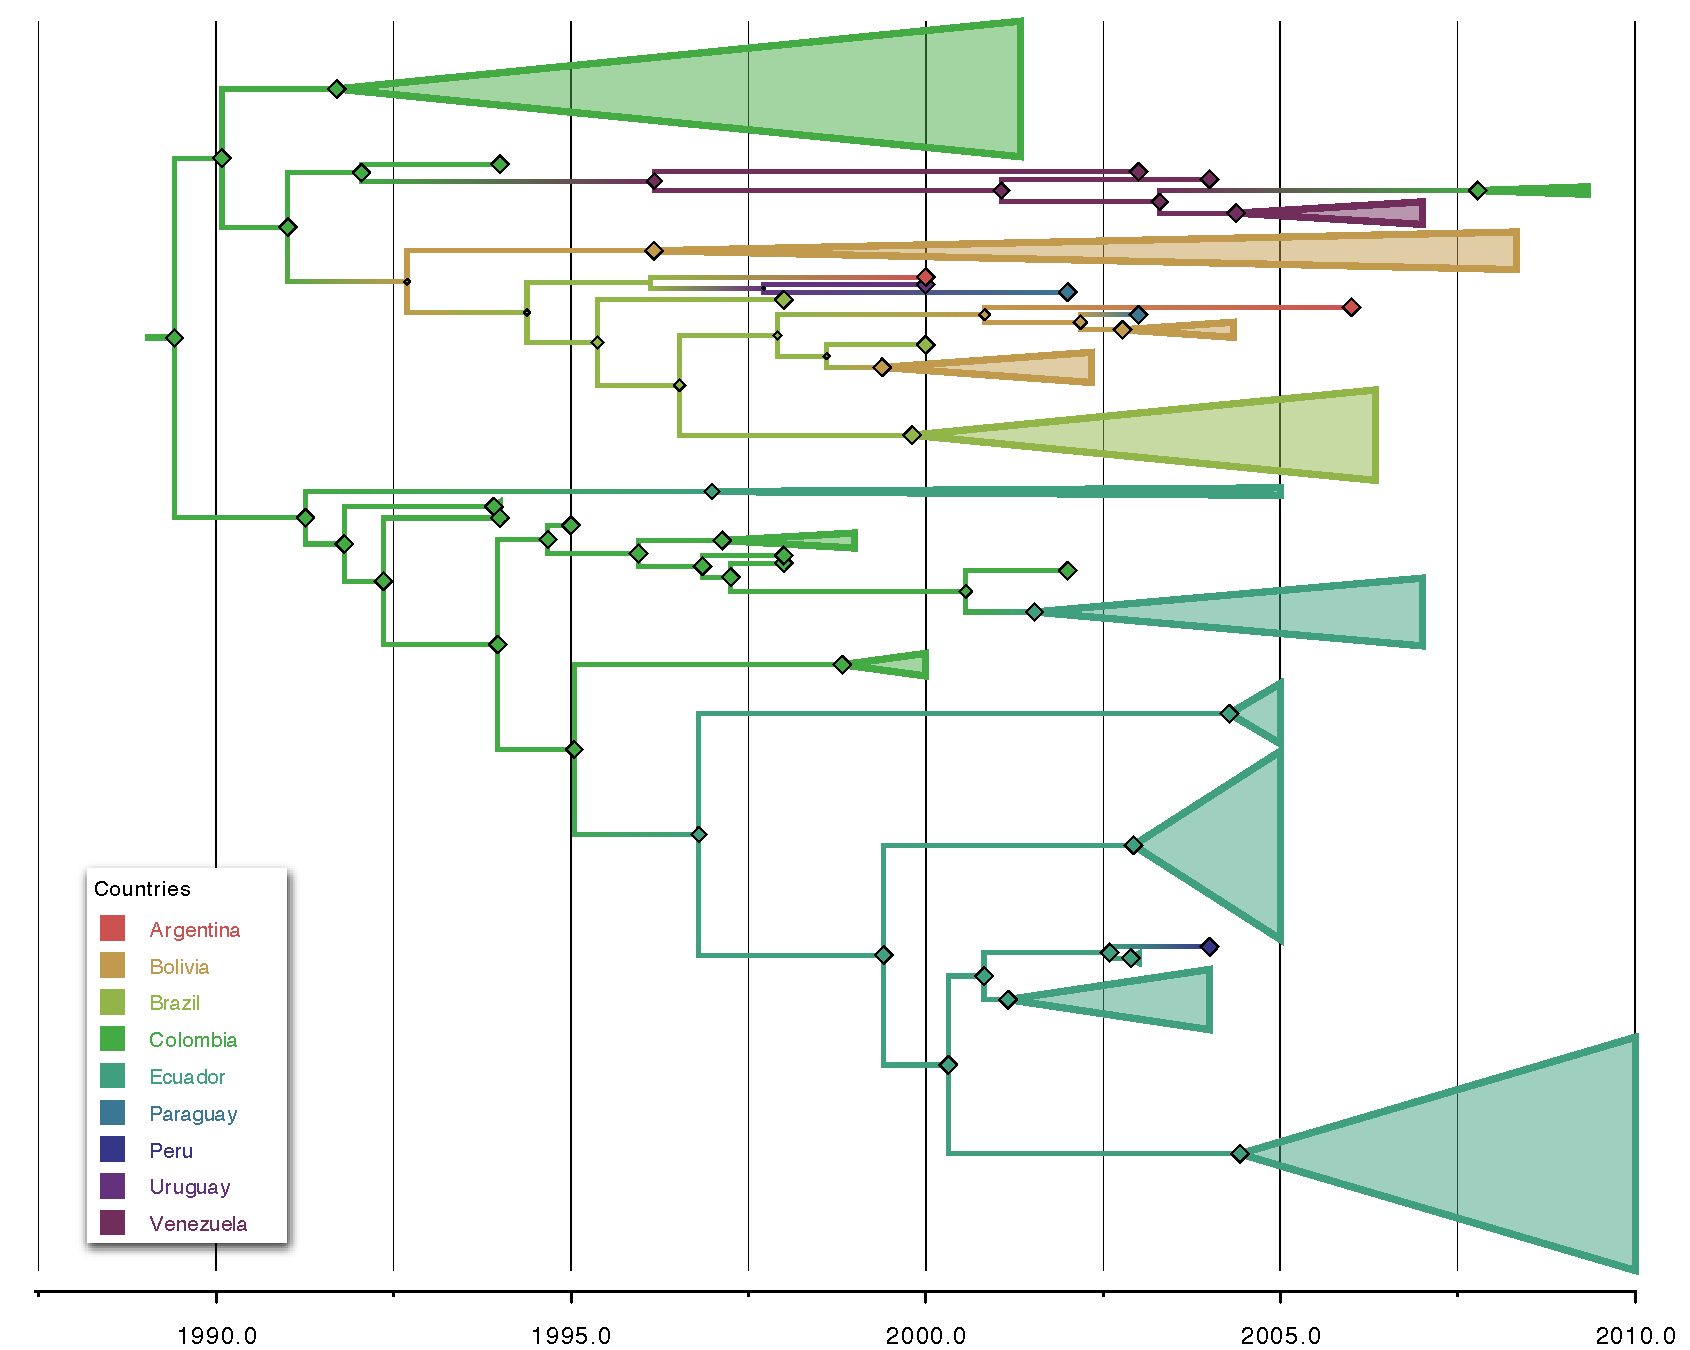
\includegraphics[scale=.60]{FIGURES/O.pdf}
\end{center}
\caption{}
\label{fig:Otree}
\end{figure}
%%%%%%%%%%%%%%%%%%%%%%%%%%
%%%%%%%%%%%%%%%%%%%%%%%%%%
\newpage
\begin{figure}[!ht]
\begin{center}
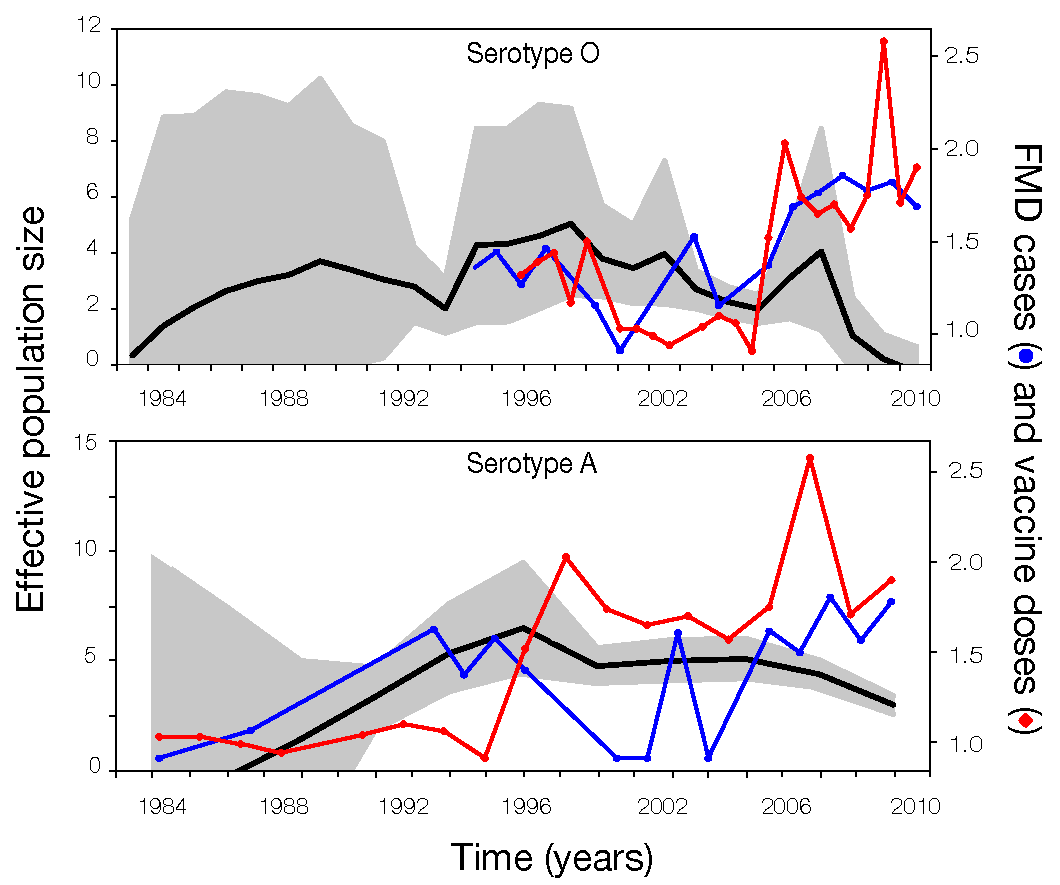
\includegraphics[scale=1.0]{FIGURES/skygrid.pdf}
\end{center}
\caption{}
\label{fig:skygrid}
\end{figure}
%%%%%%%%%%%%%%%%%%%%%%%%%%
%%%%%%%%%%%%%%%%%%%%%%%%%%
\newpage
\begin{figure}[!ht]
\begin{center}
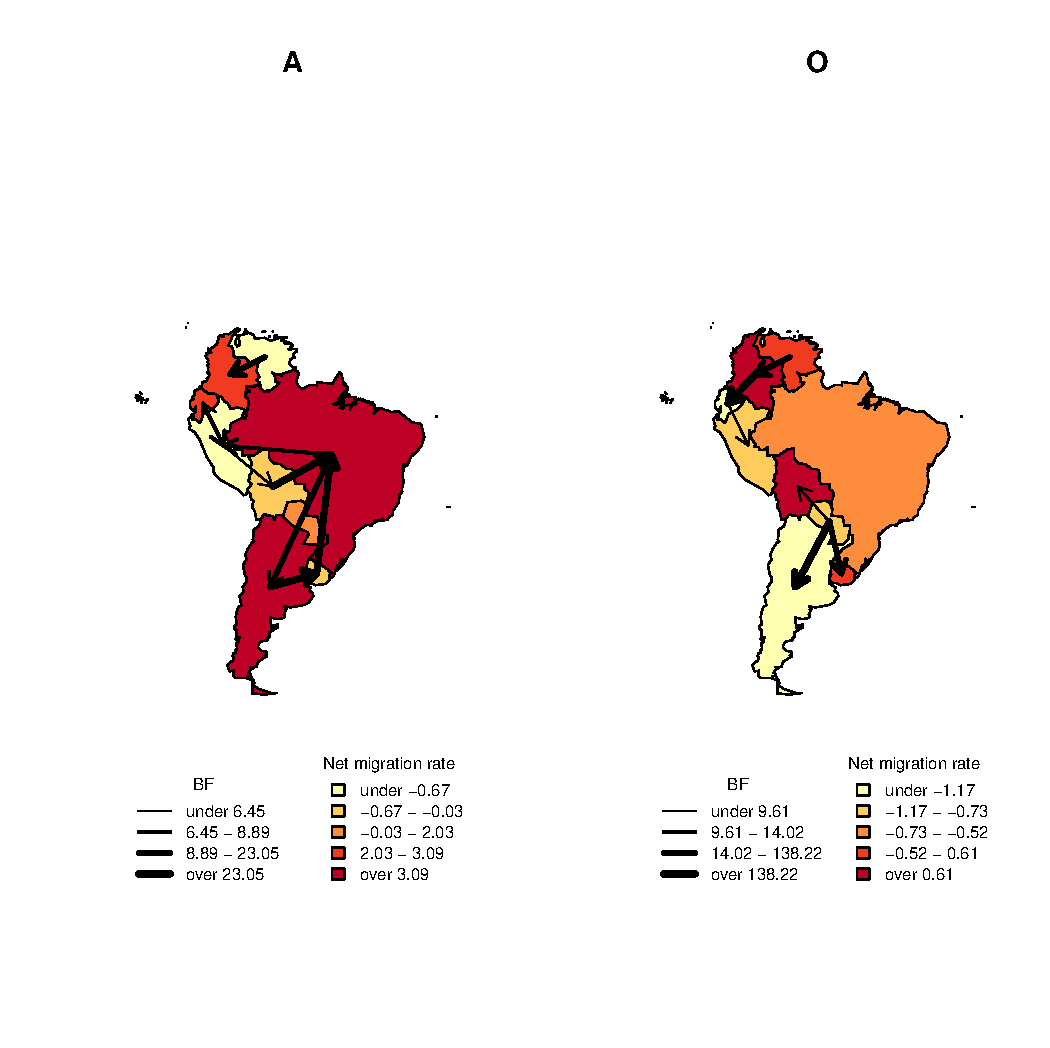
\includegraphics[scale=.85]{FIGURES/compound.pdf}
\end{center}
\caption{}
\label{fig:mj&BFs}
\end{figure}
%%%%%%%%%%%%%%%%%%%%%%%%%%
%%%%%%%%%%%%%%%%%%%%%%%%%%
\newpage
\begin{figure}[!ht]
\begin{center}
\subfigure[A --1945 ]{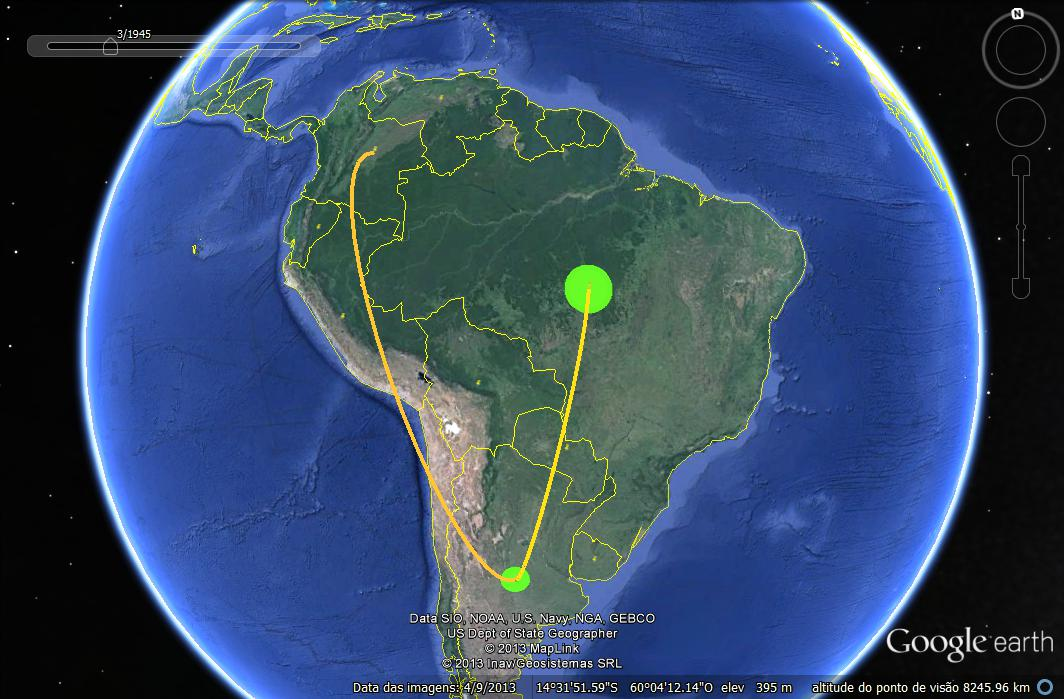
\includegraphics[scale=.20]{FIGURES/A_1945.jpg}}
\subfigure[O --1995 ]{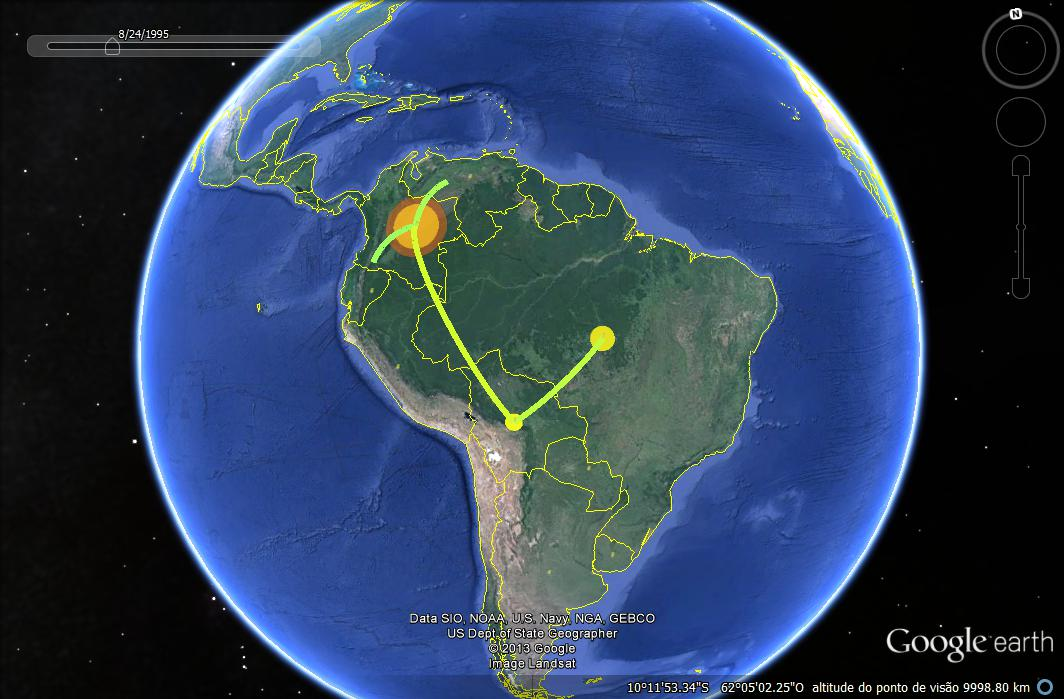
\includegraphics[scale=.20]{FIGURES/O_1995.jpg}}\\
\subfigure[A --1965 ]{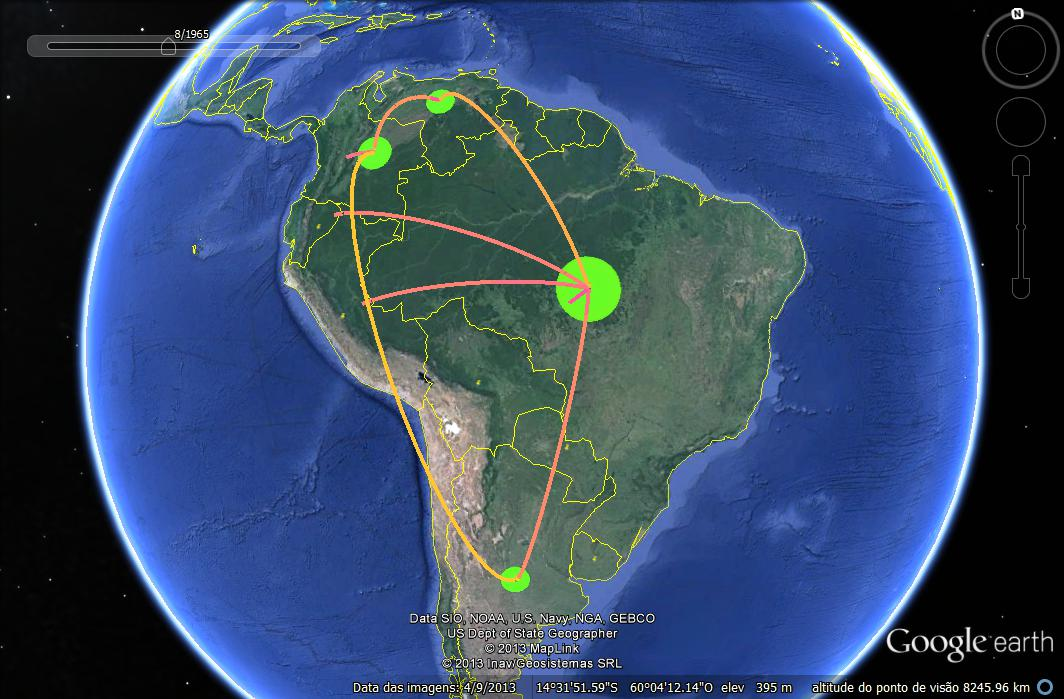
\includegraphics[scale=.20]{FIGURES/A_1965.jpg}}
\subfigure[O --2000 ]{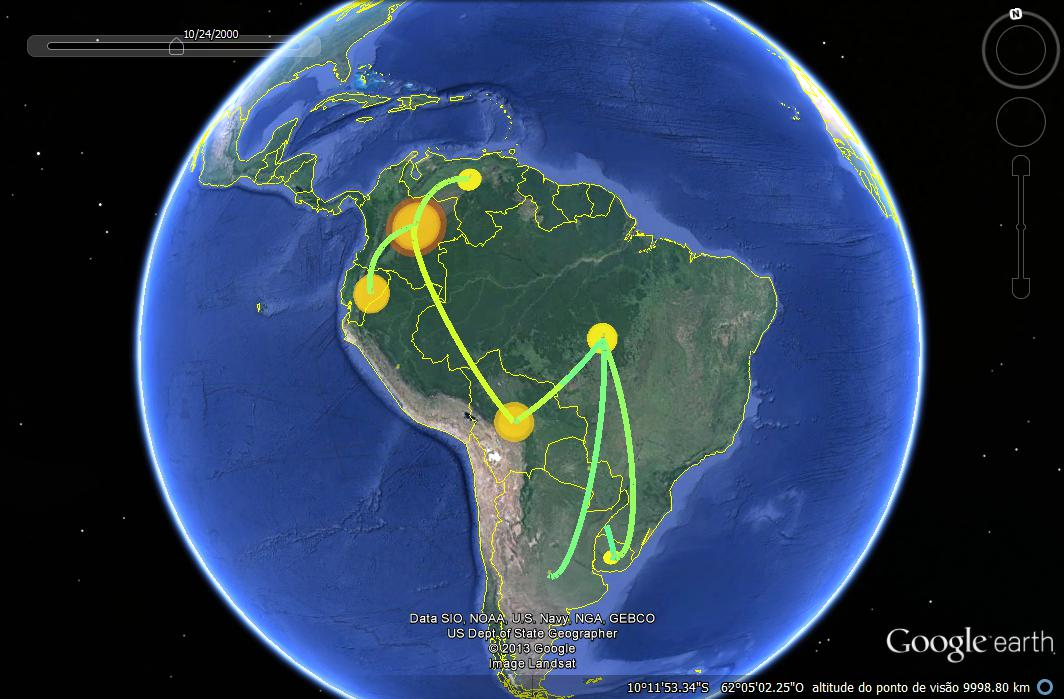
\includegraphics[scale=.20]{FIGURES/O_2000.jpg}}\\
\subfigure[A --1980 ]{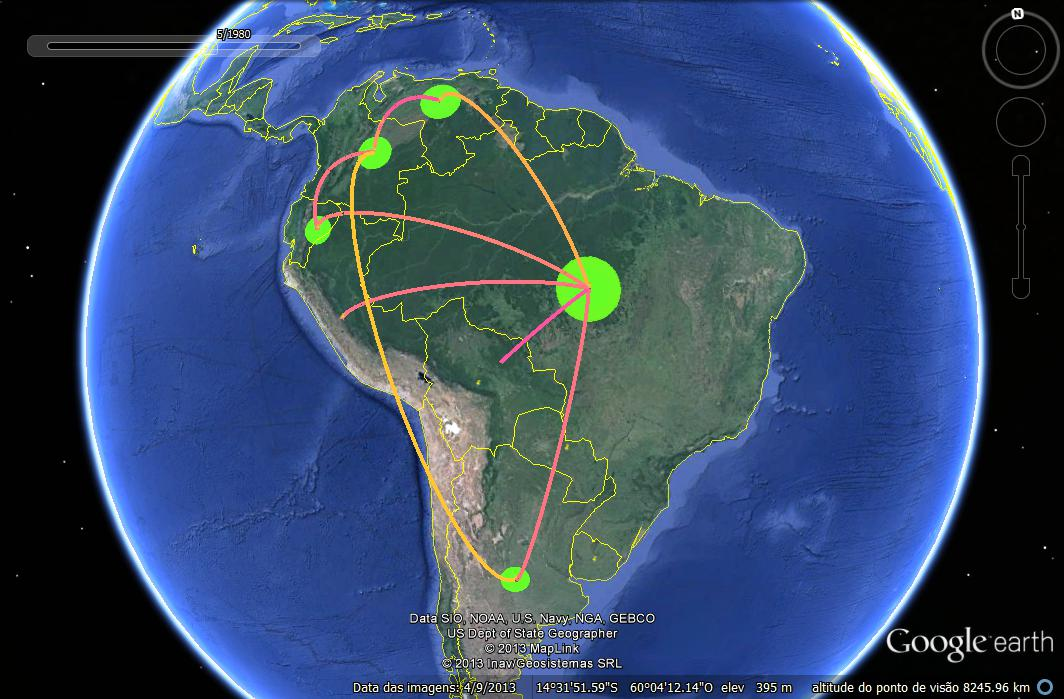
\includegraphics[scale=.20]{FIGURES/A_1980.jpg}}
\subfigure[O --2005 ]{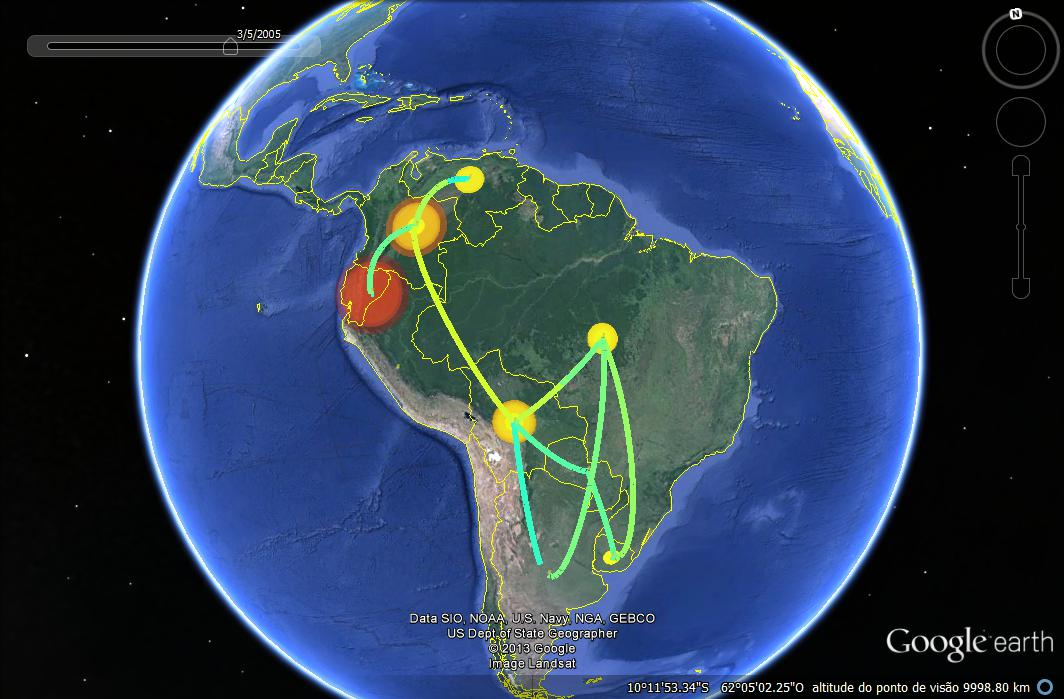
\includegraphics[scale=.20]{FIGURES/O_2005.jpg}}\\
\subfigure[A --2008 ]{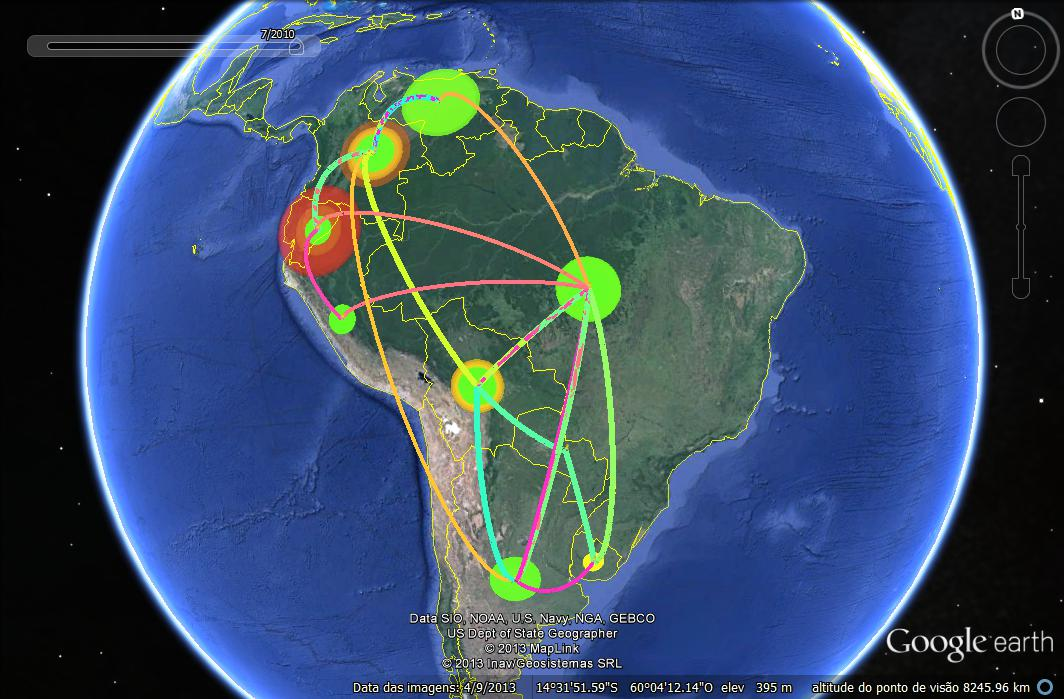
\includegraphics[scale=.20]{FIGURES/A_2008.jpg}}
\subfigure[O --2010 ]{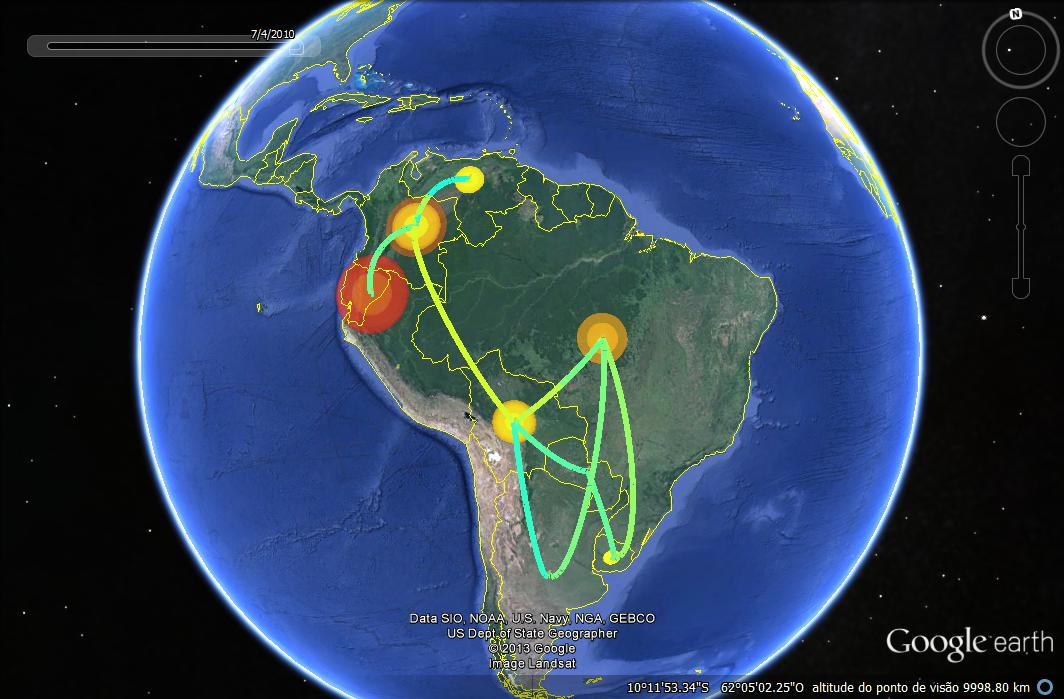
\includegraphics[scale=.20]{FIGURES/O_2010.jpg}}
\end{center}
\caption{}
\label{fig:migration}
\end{figure}
%%%%%%%%%%%%%%%%%%%%%%%%%%
%%%%%%%%%%%%%%%%%%%%%%%%%%
\newpage
\setcounter{figure}{0}
\begin{figure}[!ht]
\begin{center}
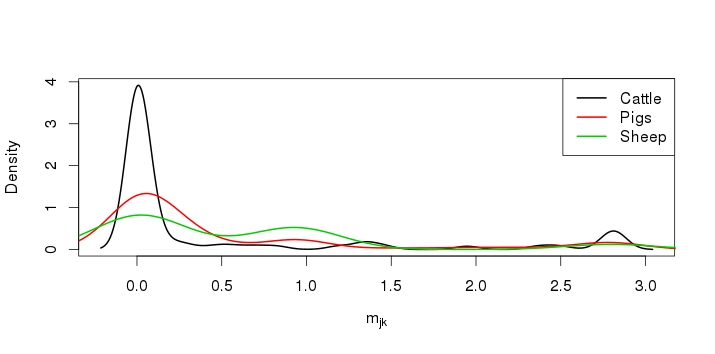
\includegraphics[scale=.5]{FIGURES/trade_info.jpeg}
\end{center}
\caption{}
\label{sfig:tradeinfo}
\end{figure}
%%%%%%%%%%%%%%%%%%%%%%%%%%
%%%%%%%%%%%%%%%%%%%%%%%%%%
% TODO: These tables are really shitty... BaTS results are strange, at least...
\newpage
\section*{Tables}
\begin{table}[!ht]
\caption{
\textbf{Spatial signal for serotype A.} 1-AI = association index; 2-PS = parsimony score; 3- Monophyletic clade size}
\begin{tabular}{cccc}
\toprule
Statistic &	Observed mean ( 95\% CI)&	Null mean ( 95\% CI)&	p-value\\
\midrule
AI$^1$	&1.56 (1.10, 2.01)& 10.75 (9.67, 11.83) &0.000\\
PS$^2$	&22.88 (22.00, 24.00)	&66.78	(63.06, 70.01)	&0.000\\
Argentina &12.31 (12.00, 14.00)	&3.45	(2.22, 5.11)	&0.001\\
MC$^3$ Brazil &10.27	(10.00, 11.00)	&2.02 (1.25, 3.00) &0.001\\
Bolivia &6.00 (6.00, 6.00)	&1.39 (1.00, 2.00)	&0.001\\
Colombia &5.11 (5.00, 6.00)	&1.10  (1.00, 1.99)	&0.001\\
Ecuador &1.00 (1.00, 1.00)	&1.00 (1.00, 1.00)	&1.000\\
Peru&1.00 (1.00, 1.00)	&1.02 (1.00, 1.00)	&1.000\\
Uruguay &5.11 (5.00, 7.00)	&1.50	(1.00, 2.03)	&0.001\\
Venezuela&1.82 (1.00, 2.00)	&1.02 (1.00, 1.08)	&0.010\\
\bottomrule
\end{tabular}
\begin{flushleft}
\end{flushleft}
\label{tab:BaTSA}
 \end{table}
%%%%%%%%%%%%%%%%%%%%%%%%
%%%%%%%%%%%%%%%%%%%%%%%%
\begin{table}[!ht]
\caption{
\textbf{Spatial signal for serotype O. } 1-AI = association index; 2-PS = parsimony score; 3- Monophiletic clade size}
\begin{tabular}{cccc}
\toprule
Statistic &	Observed mean ( 95\% CI)&	Null mean ( 95\% CI)&	p-value\\
\midrule
AI$^1$ &	0.87 (0.59, 1.19)&	11.58 (10.52, 12.67)&	0.000\\
PS$^2$ &	16.23 (15.00, 17.00)&	71.23 (68.17, 73.97)&	0.000\\
MC$^3$ Ecuador& 13.00 (13.00, 13.00)&	1.34 (1.00, 2.00)&	0.001\\
Peru&	1.00 (1.00, 1.00)&	1.01 (1.00, 1.00)&	1.000\\
Colombia&	1.00 (1.00, 1.00)&	1.00 (1.00, 1.00)&	1.000\\
Venezuela&	6.00 (6.00, 6.00)&	1.28 (1.00, 2.00)&	0.001\\
Bolivia &	1.00 (1.00, 1.00)&	1.00 (1.00, 1.00)&	1.000\\
Brazil&	19.00 (19.00, 19.00)&	2.19 (1.66, 3.03)&	0.001\\
Paraguay&	39.40 (31.00, 58.00)&	4.67 (3.43, 6.39)&	0.001\\
Argentina&	1.00 (1.00, 1.00)&	1.00 (1.00, 1.00)&	1.000\\
Uruguay&	4.00 (4.00, 4.00)&	1.06 (1.00, 1.32)&	0.001\\
\bottomrule
\end{tabular}
\begin{flushleft}
\end{flushleft}
\label{tab:BaTSO}
 \end{table}
%%%%%%%%%%%%%%%%%%%%%%%%
%%%%%%%%%%%%%%%%%%%%%%%%
\begin{table}[!ht]
\caption{
\textbf{Spatial model selection results for serotype A. } GUY's SHARE.}
\begin{tabular}{cccccc}
\toprule
Model & AICM  & PS    & SS\\
\midrule
Cattle	&24179.81	&-12587.52	&-12590.37\\
Cattle-Freq	&24295.23	&-12650.74	&-12652.75\\
Distance	&24139.74	&-12561.42	&-12565.78\\
Pig	&24149.17	&-12563.14	&-12568.15\\
Pig-Freq	&24260.55	&-12626.62	&-12633.73\\
Sheep	& {{ \bf 24113.82}}	& {{\bf -12542.57}}	& {{\bf -12548.95}}\\
Sheep-Freq	&24187.00	&-12580.01	&-12584.59\\
Uniform	&24157.43	&-12562.42	&-12567.60\\
\bottomrule
\end{tabular}
\begin{flushleft}
\end{flushleft}
\label{tab:predA}
 \end{table}
%%%%%%%%%%%%%%%%%%%%%%%%
%%%%%%%%%%%%%%%%%%%%%%%%
\begin{table}[!ht]
\caption{
\textbf{Spatial model selection results for serotype O. } GUY's SHARE. 1-Base frequencies for each state set at the relative representations in the data set. }
\begin{tabular}{cccc}
\toprule
Model	&AICM	&PS	&SS\\
\midrule
Cattle	&15581.07	&{{ \bf -8293.99}}	&-8300.01\\
Cattle-Freq$^1$	&15557.28	&-8301.17	&-8306.27\\ % Is this right? I mean Freq stands for sampling-corrected  
Distance	& {{\bf 15562.60 }}	&-8294.19	& {{ \bf -8298.52}} \\
Pig	&15593.10	&-8308.99	&-8312.37\\
Pig-Freq	&15600.41	&-8327.04	&-8334.30\\
Sheep	&15572.90	&-8299.84	&-8304.83\\
Sheep-Freq	&15578.06	&-8308.06	&-8313.53\\
Uniform	&15572.63	&-8299.04	&-8306.21\\
\bottomrule
\end{tabular}
\begin{flushleft}
\end{flushleft}
\label{tab:predO}
 \end{table}
%%%%%%%%%%%%%%%%%%%%%%%%
%%%%%%%%%%%%%%%%%%%%%%%%
\begin{table}[!ht]
\caption{
\textbf{Inferred root locations for each predictor for both serotypes.} We present most probable country of origin inferred using each predictor, with associated probabilities inside parentheses. 1- Uniform, all rates equal prior.
}
\begin{tabular}{lcc}
\toprule
Model & Serotype A & Serotype O \\
\midrule
Distance & Peru (0.94) & Colombia (0.92)\\
Sheep    & Brazil (0.83) &Colombia (0.98)\\
Pig      & Colombia (0.99) &Colombia (0.52)\\
Uniform$^1$  & Peru (0.94) &Colombia (0.92)\\
Cattle   & Peru (0.92) &Colombia (0.95)\\
Sheep-Freq & Peru (0.90)&Colombia (0.86)\\
Pig-Freq & Colombia (0.51) &Colombia (0.57)\\
Cattle-Freq & Peru (0.89)& Colombia (0.97)\\
 \bottomrule
\end{tabular}
\begin{flushleft}
\end{flushleft}
\label{tab:roots}
 \end{table}
 % TODO: check these results again with the new runs
%%%%%%%%%%%%%%%%%%%%%%%%
%%%%%%%%%%%%%%%%%%%%%%%%
\newpage
\begin{table}[!ht]
\caption*{\textbf{Table S1. Model selection for tree (coalescent) model and clock for both serotypes.}  ULN= uncorrelated log-normal; UCED = uncorrelated exponential . Best fitting models (highest log-likelihood) are highlighted in bold.}
\begin{tabular}{cccccc}
\toprule
Serotype	&Coalescent	&Clock	&Log-Likelihood$^{1}$\\
\midrule
A	&Constant	&ULN	&-12285\\
A	&Skyride 	&ULN	&\textbf{-12274}\\
A	&Constant	&UCED	&-12316\\
A	&Skyride 	&UCED	&-12307\\
A       &Skyride       &STRICT &-12308\\
O	&Constant	&ULN	&-8087\\
O	&Skyride 	&ULN	&-8082\\
O	&Constant	&UCED	&-8090\\
O	&Skyride 	&UCED	&\textbf{-8069}\\
O       &Skyride       &STRICT &-8125\\
\bottomrule
\end{tabular}
\begin{flushleft}
\end{flushleft}
\label{stab:treeclockselection}
 \end{table}
%%%%%%%%%%%%%%%%%%%%%%%%
%%%%%%%%%%%%%%%%%%%%%%%%
\end{document}
